\section{Azioni preliminari}
	%Descrizione delle azioni per entrare nell'applicazione quali:
	%sito dell'applicazione
	%login
	%pagine inerenti l'applicazione (praticamente tutti quello che esiste gia e che NON abbiamo fatto noi)
	%il cambio lingua va fatto qua??
	%	\gls{bbb}
DeGeOP è sviluppato su una single page che risulta essere parte integrante dell'attuale applicazione di \riskapp{}.
\\
Per accedere a DeGeOP, l'utente deve quindi effettuare una serie di operazioni:
\begin{itemize}
	\item aprire la \mglo{VirtualBox}{virtual box} fornita da \riskapp{};
	\item aprire il \mglo{Browser}{browser};
	\item effettuare l'accesso al sito di \riskapp{} cliccando sul segnalibro presente sulla barra dei segnalibri, utilizzando le seguenti credenziali:
	\begin{itemize}
		\item nome utente: admin;
		\item password: admin.
		\begin{figure}[H]
		\centering
		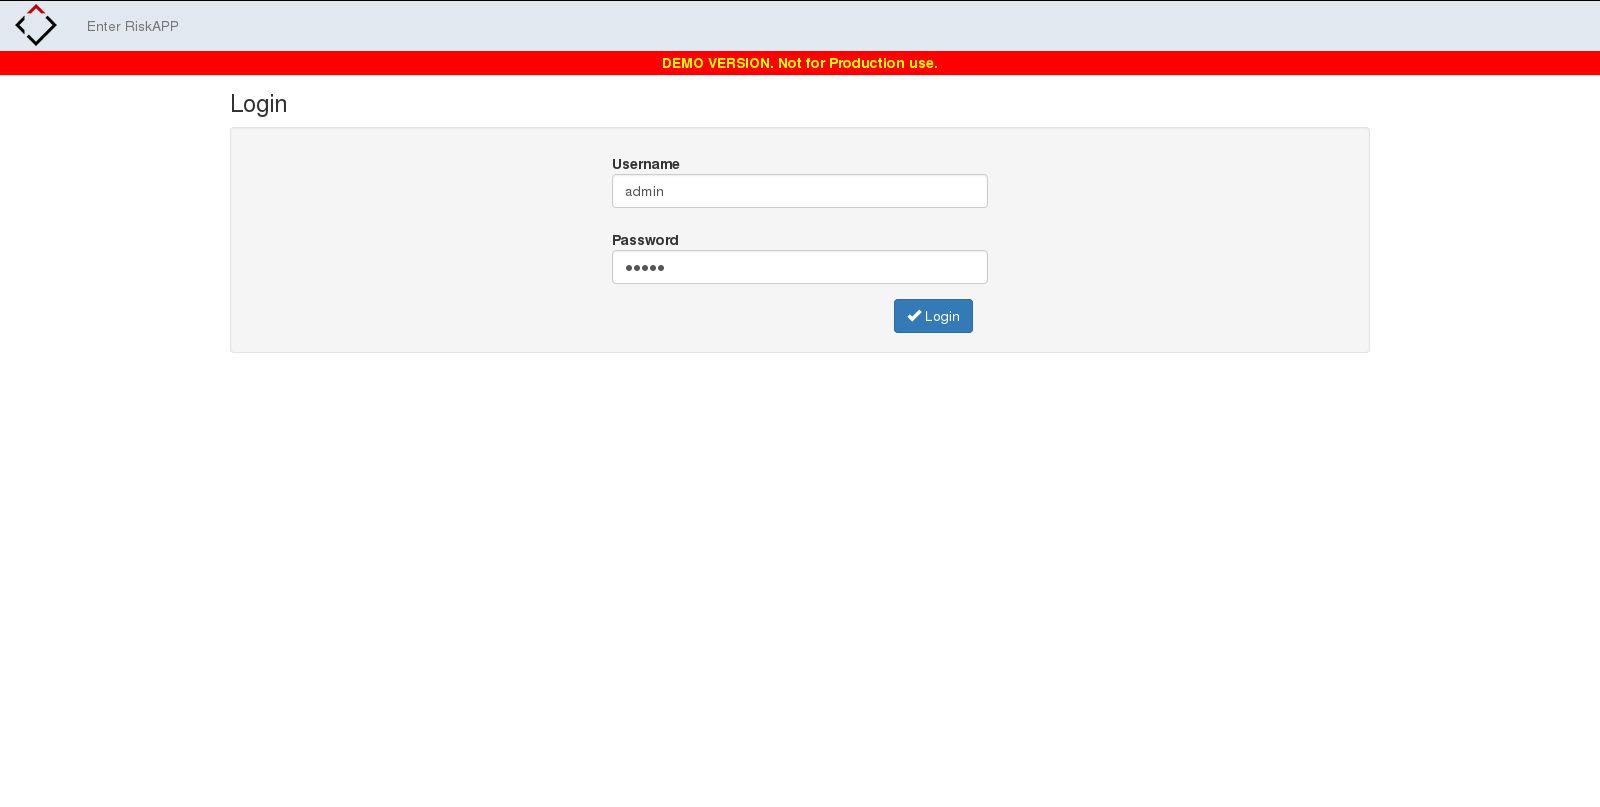
\includegraphics[width=\textwidth]{img/accessoDeGeOP/s1-login.png}
		\caption{Pagina di Login in RiskApp}
		\end{figure}
		
	\end{itemize}
	\item scegliere un cliente cliccando sul relativo pulsante "Edit";
		\begin{figure}[H]
		\centering
		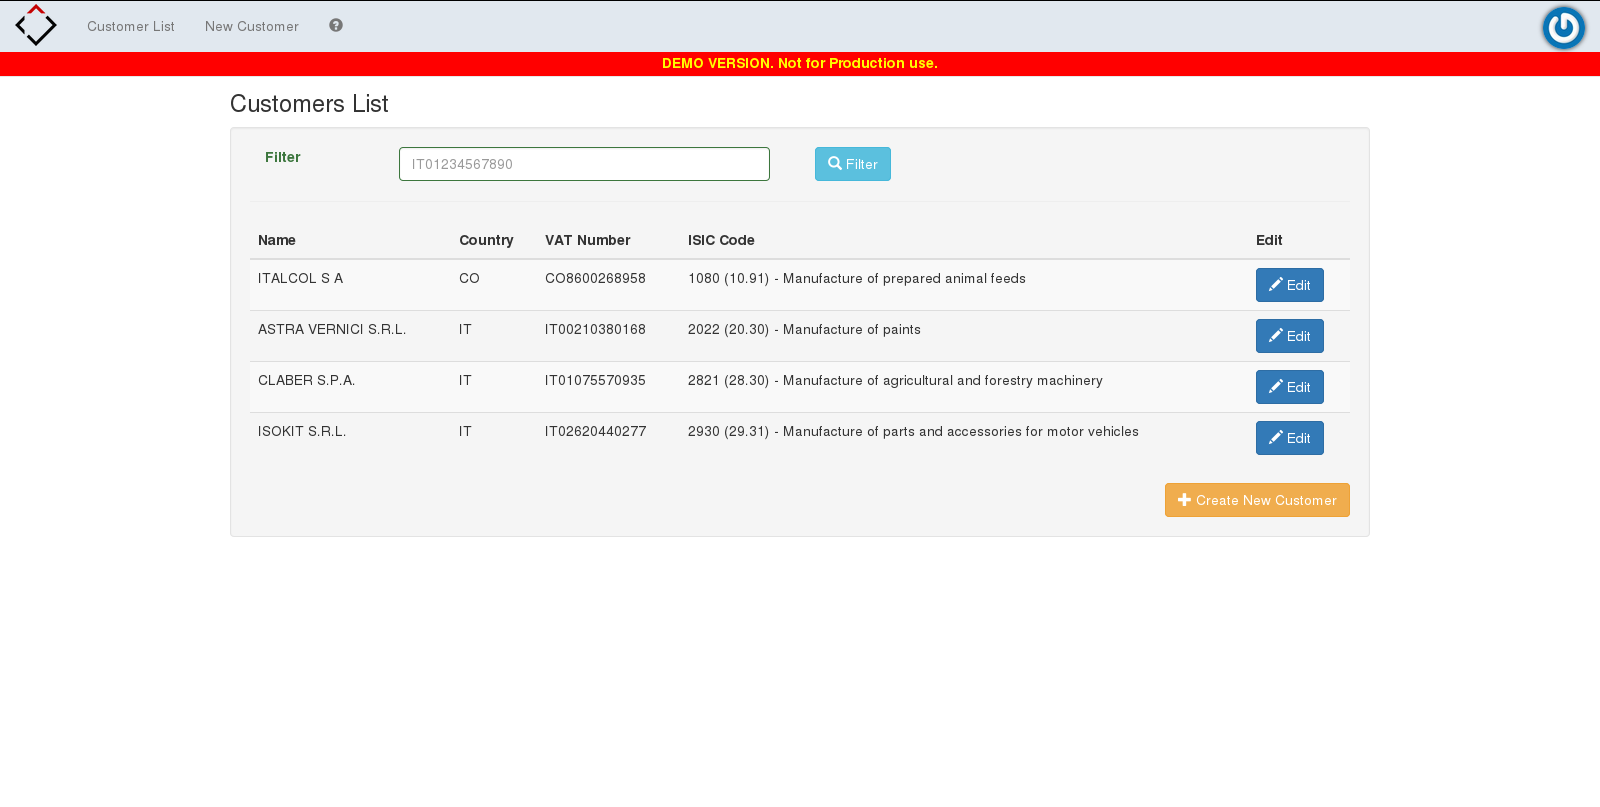
\includegraphics[width=\textwidth]{img/accessoDeGeOP/s2-select_customer.png}
		\caption{Scelta cliente in RiskApp}
		\end{figure}
	\item cliccare sulla scheda di menu denominata "Customer";
		\begin{figure}[H]
		\centering
		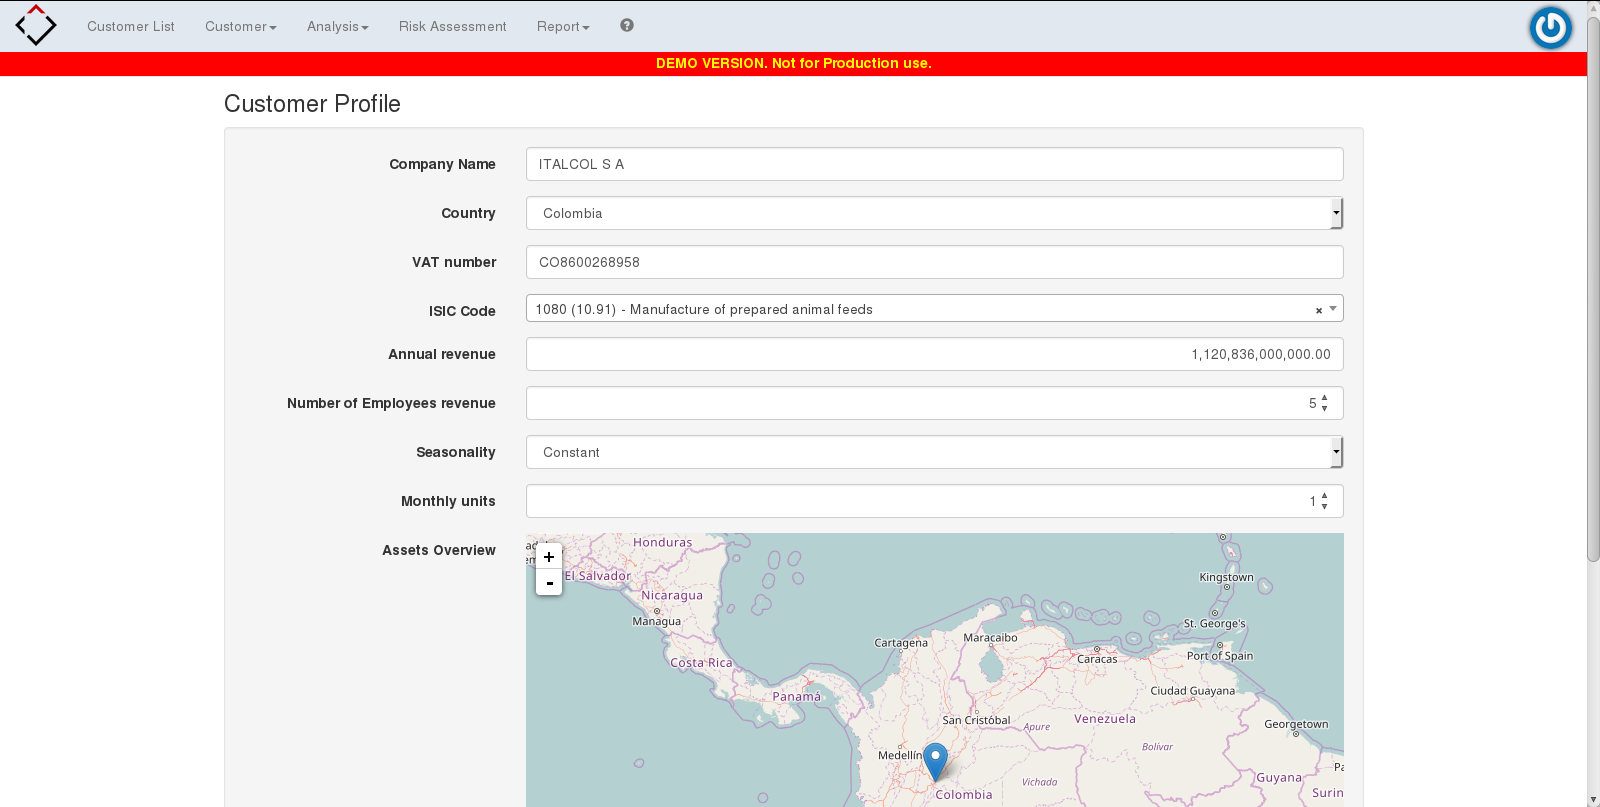
\includegraphics[width=\textwidth]{img/accessoDeGeOP/s3-customer_dashboard.png}
		\caption{Scheda di menu "Customer" in RiskApp}
		\end{figure}
	\item nel menu a tendina che compare, scegliere la voce "Processes";
		\begin{figure}[H]
		\centering
		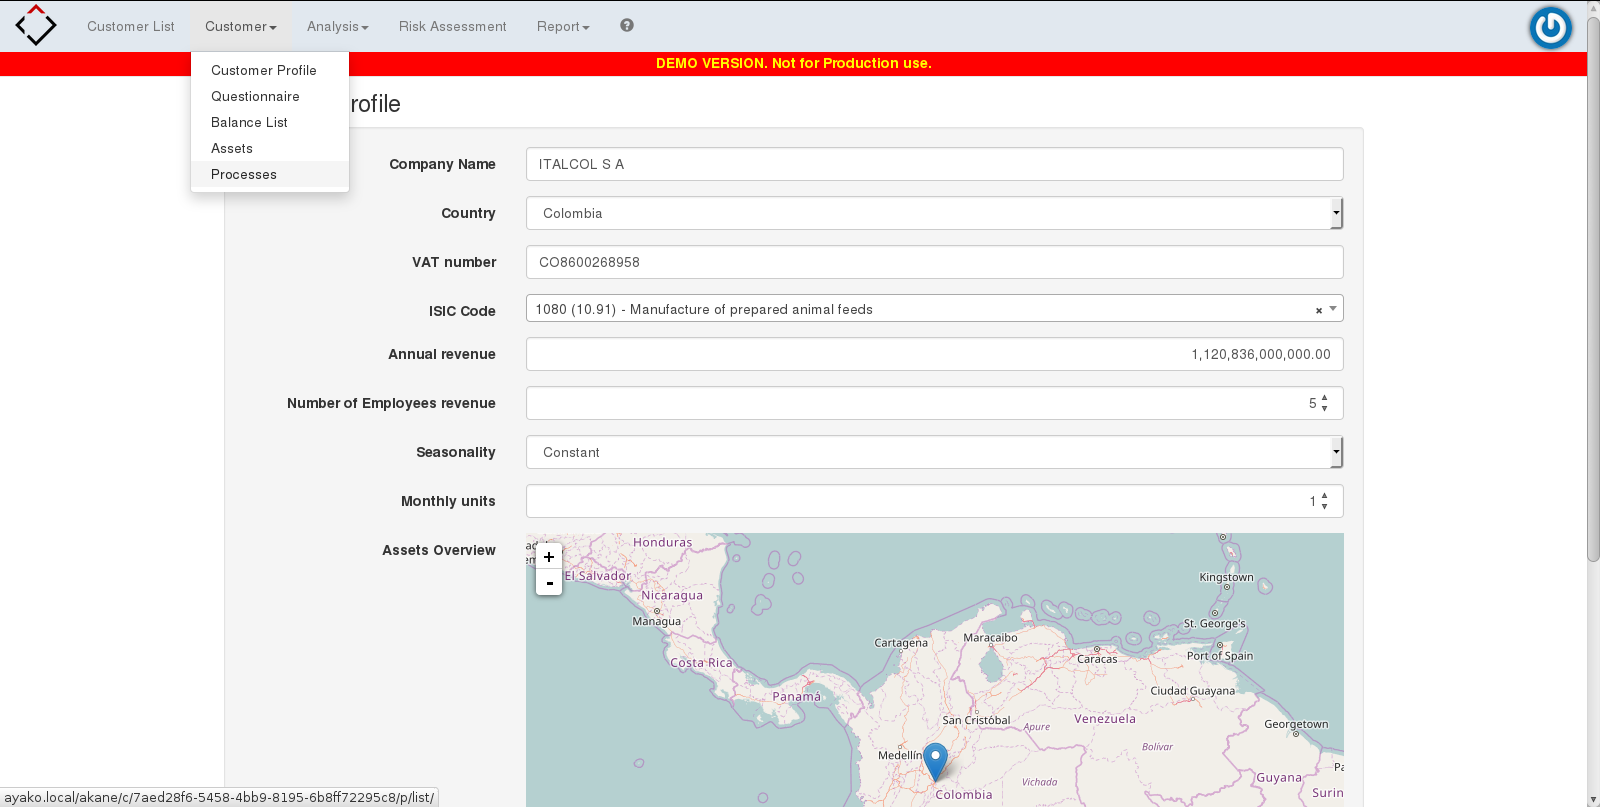
\includegraphics[width=\textwidth]{img/accessoDeGeOP/s4-select_menu_voice.png}
		\caption{Voce "Process" in RiskApp}
		\end{figure}
	\item scegliere un processo da modificare cliccando sul relativo pulsante "Edit";
		\begin{figure}[H]
		\centering
		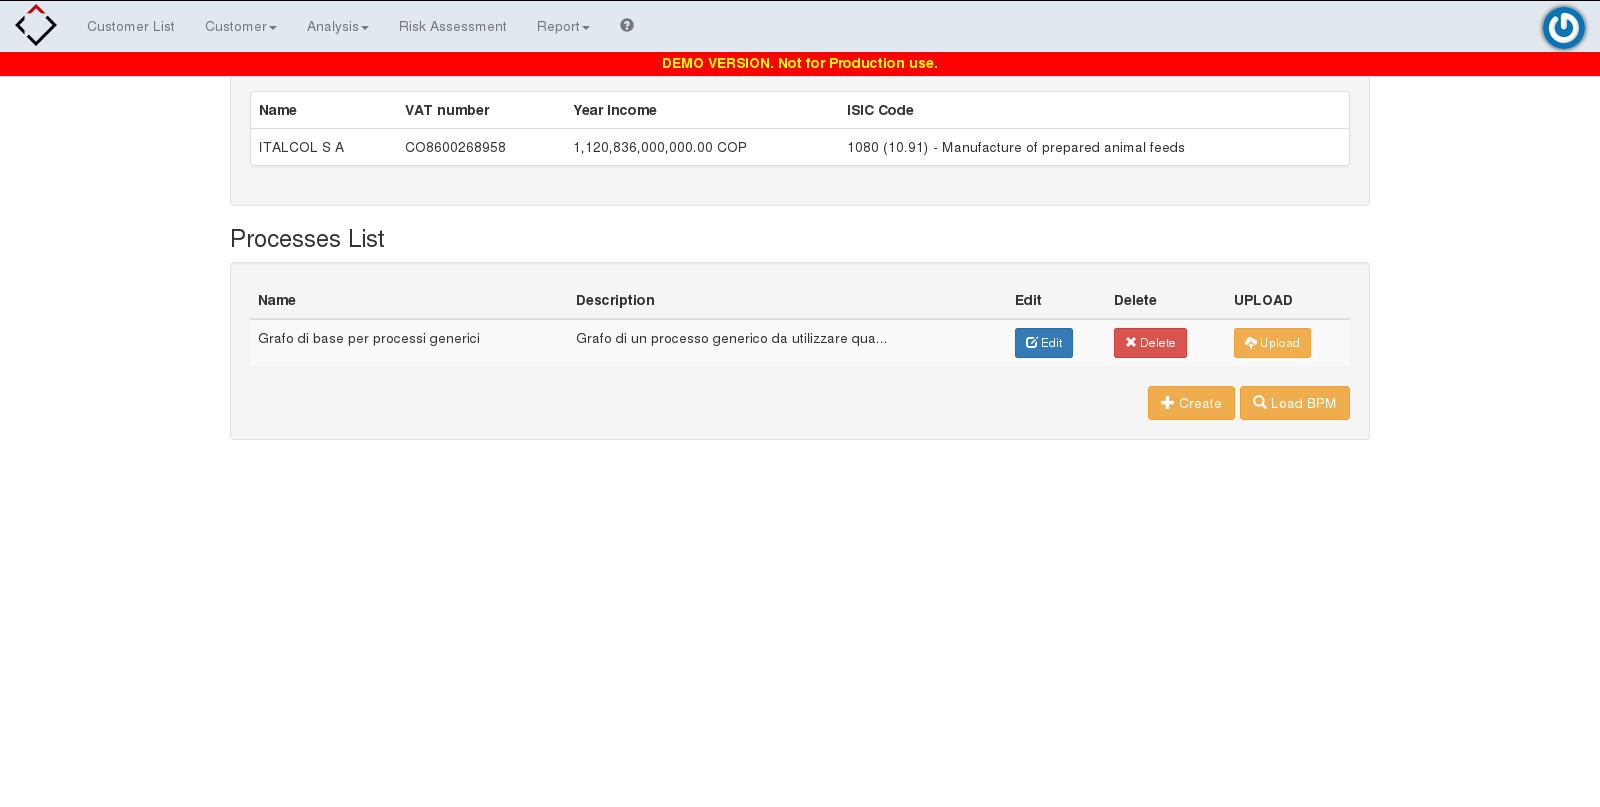
\includegraphics[width=\textwidth]{img/accessoDeGeOP/s5-select_process.png}
		\caption{Scelta processo in RiskApp}
		\end{figure}
	\item sei giunto alla single page DeGeOP.
	\\Per la precisione il prodotto DeGeOP consiste nella la parte sottostante alla linea rossa. Segue quindi uno screenshot dell'intera applicazione.
		\begin{figure}[H]
		\centering
		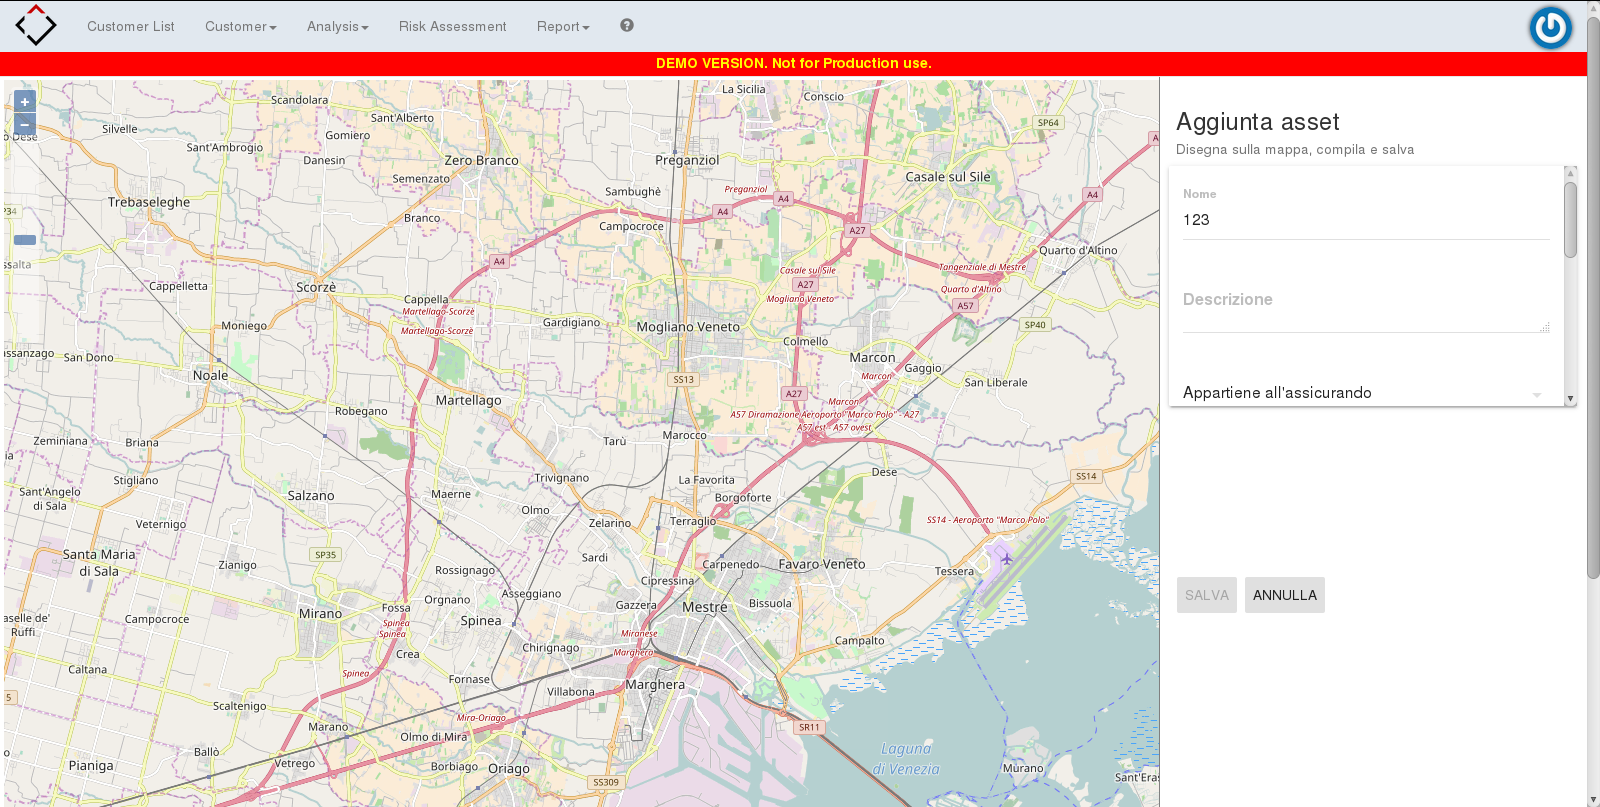
\includegraphics[width=\textwidth]{img/accessoDeGeOP/s6-DeGeOP.png}
		\caption{DeGeOP}
		\end{figure}
\end{itemize}
